\documentclass[twocolumn,10pt]{article}
\usepackage[letterpaper,left=1.95cm,right=1.95cm,top=2.5cm,bottom=3.16cm]{geometry} % Márgenes y demás
\usepackage{natbib}
\usepackage{hyperref}
\usepackage{enumitem}
\usepackage{balance}
\usepackage{booktabs}
\usepackage[utf8]{inputenc}
\usepackage{wasysym} % symbols
\usepackage{amssymb} % symbols
\usepackage{abstract}
\usepackage{parskip}
\usepackage{hyperref}
\usepackage{titlesec}
\usepackage{xcolor}
\usepackage{natbib}
\usepackage{float}
\usepackage{graphicx}
\usepackage{fancyhdr}
\usepackage{titling}
\usepackage{caption}
\usepackage[document]{ragged2e}
\usepackage[affil-sl]{authblk} 
\usepackage{mathptmx}  %Times new Roman

\setlength{\columnsep}{1cm}
\renewcommand{\refname}{BIBLIOGRAFÍA}
\renewcommand{\figurename}{Fig.}
\renewcommand{\tablename}{Tabla.}
\renewcommand{\abstractname}{RESUMEN}

% Keywords command
\providecommand{\keywordsSpan}[1]
{
  \small	
  \textbf{\textit{Palabras Clave:}} #1
}

\providecommand{\keywordsEng}[1]
{
  \small	
  \textbf{\textit{Keywords:}} #1
}


%%%%%%%% FORMATO DE LAS SECCIONES Y SUBSECCIONES %%%%%
\titleformat{\section} 
	{\normalfont\large\bfseries}{\makebox[30pt][l]{\thesection}}{0pt}{} 
\titleformat{\subsection} 
	{\normalfont\large\bfseries }{\makebox[30pt][l]{\thesubsection}}{0pt}{}
\renewcommand\thesection{\arabic{section}.}
\renewcommand\thesubsection{\thesection\arabic{subsection}}
%%%%%%%% FORMATO DE LAS SECCIONES Y SUBSECCIONES %%%%%


	
\makeatletter
\long\def\@makecaption#1#2{
\vskip\abovecaptionskip
\sbox\@tempboxa{#1. #2}
\ifdim \wd\@tempboxa >\hsize
#1. #2\par
\else
\global \@minipagefalse
\hb@xt@\hsize{\hfil\box\@tempboxa\hfil}
\fi
\vskip\belowcaptionskip}
\makeatother


\pagestyle{fancyplain}% <- pagestyle fancyplain

\fancyfoot[C]{}
\renewcommand\plainheadrulewidth{.4pt}% headrule on plain pages
%\fancyhf{}
\rhead{Semestre 4 Año 2026}
\lhead{Estadística Bayesiana}
\rfoot{\thepage}

\date{}
  %%Llama el archivo de los estilos

%%%%%%% ENCABEZADO %%%%%%%%%%%%%%%%%%%%

{\title{\fontsize{16}{16}\selectfont
\vspace*{-0.7cm}
\textbf{
Predecir lo Impredecible: Un Enfoque de Estadística Bayesiana para Estimar Victorias en CS:GO
} \\[0.2cm]
\fontsize{12}{12}\selectfont
\textbf{Predicting the Unpredictable: A Bayesian Statistics Approach to Estimate Win Probability in CS:GO}\\[0.2cm]}
}

\author[1,*]{\fontsize{10pt}{10pt}\selectfont \textbf{Julián Duarte}}
\author[2]{\textbf{Julián Jiménez}}
\author[3]{\textbf{Tomás Rincón}}


\affil[1]{
\fontsize{8pt}{8pt}\selectfont Pregrado Ciencia de Datos Universidad Externado, Bogotá - Colombia}
\fontsize{8}{8}
\affil[2]{Pregrado Ciencia de Datos Universidad Externado, Bogotá - Colombia}
\affil[3]{Pregrado Ciencia de Datos Universidad Externado, Bogotá - Colombia \vspace{0.2cm}} 
\affil[*]{julian.duarte2@est.uexternado.edu.co \\
julian.jimenez5@est.uexternado.edu.co \\
juan.rincon14@est.uexternado.edu.co}

%%%%%%%%%%%%%%%%%%%%%%%%%%%%%%%%% INICIO DEL DOCUMENTO
%%%%%%%%%%%%%%%%%%%%%%%%%%%%%%%%%%%%%%%%%%%%%%%%%%%%%%%%%%%%%%%%%%%%%%%

\begin{document}

\twocolumn[
  \begin{@twocolumnfalse}
    \maketitle

    \begin{center}
        \textbf{RESUMEN}
    \end{center}
    Este proyecto de investigación propone una forma novedosa y práctica de estimar quién ganará en partidas profesionales de \textit{Counter-Strike} (CS:GO/CS2), utilizando la estadística bayesiana. A diferencia de los modelos tradicionales que arrojan un simple porcentaje de \textit{gana o pierde}, nuestro enfoque permite medir objetivamente la incertidumbre; es decir, nos dice qué tan seguros estamos de esa predicción. Al integrar factores decisivos —como el escenario o mapa elegido, la habilidad técnica base y la capacidad de impacto de los equipos—, construimos una herramienta matemática transparente y fácil de entender. Esta metodología no solo enriquece la analítica deportiva, sino que dota a organizaciones profesionales e inversores de un instrumento claro para gestionar el riesgo y tomar decisiones sólidas en un ecosistema donde cualquier detalle cambia el resultado final.
    \vspace{0.2cm}

    \keywordsSpan{Esports, Estadística Bayesiana, CS:GO, Gestión de Riesgo, Incertidumbre.}
    
    \vspace{0.6cm}

    \begin{center}
        \textbf{ABSTRACT}
    \end{center}
    This research project proposes a novel and practical approach to estimating who will win in professional \textit{Counter-Strike} (CS:GO/CS2) matches using Bayesian statistics. Unlike traditional models that return a simple \textit{win or lose} percentage, our approach objectively measures uncertainty; that is, it tells us how confident we are in that prediction. By integrating deciding factors—such as the chosen stage or map, technical rating, and impact metrics—we build a transparent and easily understood mathematical tool. This methodology not only enriches sports analytics but also provides professional organizations and investors with a clear instrument to manage risk and make solid decisions in an ecosystem where any detail changes the final outcome.
    \vspace{0.2cm}

    \keywordsEng{Esports, Bayesian Statistics, CS:GO, Risk Management, Uncertainty.}
    \vspace{0.8cm}
  \end{@twocolumnfalse}
]

\thispagestyle{fancyplain} % Restaurado del estilo oficial

\section{INTRODUCCIÓN}

\justifying
El ecosistema competitivo de los deportes electrónicos (\textit{esports}), liderado por títulos como \textit{Counter-Strike: Global Offensive} (CS:GO) y su sucesor CS2, ha alcanzado una madurez estadística que exige herramientas de análisis de riesgo más allá del simple pre-dictamen binario. Históricamente, la literatura académica y las aplicaciones comerciales han dependido de clasificadores tradicionales basados en el aprendizaje automático (\textit{Machine Learning}), los cuales, si bien logran precisiones (\textit{accuracy}) aceptables, tienden a ignorar la naturaleza estocástica del juego al proporcionar predicciones secas sin un margen de error definido. En respuesta a esta deficiencia, la presente investigación fundamenta el diseño de un modelo basado en \textbf{Estadística Bayesiana} para estimar la probabilidad posterior de victoria, aportando una cuantificación explícita de la incertidumbre epistémica. 

La problemática central identificada tras una revisión sistemática en bases de datos indexadas como \textbf{Web of Science (WoS)} y \textbf{Scopus} — utilizando una cadena de búsqueda consolidada centrada en \texttt{('win probability' AND 'Bayesian')} — revela un vacío crítico en la calibración probabilística. Los modelos dominantes sufren de \textit{overconfidence} (sobreconfianza), especialmente en encuentros de alta paridad técnica, donde el azar y la asimetría de los mapas (\textit{map pool}) juegan un papel determinante que los modelos frecuentistas no logran regularizar eficazmente. Delimitando el problema mediante el marco \textbf{PICOC}, se han establecido los objetivos de desarrollar e implementar un sistema predictivo que logre una estimación calibrada, integrando variables de habilidad técnica (Rating) e impacto táctico. El resto del manuscrito se organiza de la siguiente manera: la sección 2 detalla el planteamiento del problema, junto con la pregunta y justificación; la sección 3 detalla los objetivos del proyecto; la sección 4 detalla todo el analisis exploratorio de los datos y respectivo proceso de su tratamiento.

\subsection{Marco PICOC}
\begin{table}[H]
\centering
\resizebox{\linewidth}{!}{%
\begin{tabular}{|l|p{6cm}|}
\hline
\textbf{Componente} & \textbf{Descripción Aplicada} \\ \hline
\textbf{P} (Población) & Partidas profesionales de CS:GO y CS2 en torneos oficiales (Major, ESL, BLAST). \\ \hline
\textbf{I} (Intervención) & Implementación de modelos de Regresión Logística Bayesiana Jerárquica. \\ \hline
\textbf{C} (Comparación) & Clasificadores frecuentistas (Random Forest, XGBoost) y Sistemas de Ranking (ELO, Glicko-2). \\ \hline
\textbf{O} (Outcome) & Estimación de probabilidad posterior, Calibración (ECE) y Cuantificación de Incertidumbre (HDI). \\ \hline
\textbf{C} (Contexto) & Ecosistema de Esports profesional global durante el periodo 2015--2026. \\ \hline
\end{tabular}%
}
\caption{Delimitación PICOC de la investigación.}
\label{tab:picoc}
\end{table}

\subsection{Estrategia de Búsqueda y Selección (Entrega 3.2)}
Se realizó una búsqueda estructurada en las principales bases de datos indexadas (Scopus e IEEE Xplore) utilizando la cadena: \texttt{('esports' OR 'Counter-Strike') AND ('win probability' OR 'match prediction') AND ('Bayesian' OR 'probabilistic')}. Los criterios de inclusión se centraron en artículos empíricos (2015-2026) que reporten métricas de evaluación probabilística.

\section{PLANTEAMIENTO DEL PROBLEMA}

\subsection{Presentación del Problema}

Los deportes electrónicos (\textit{esports}), y en especial el juego \textit{Counter-Strike} (CS:GO/CS2), se caracterizan por ser muy impredecibles. Hay decenas de tácticas en juego y cualquier detalle, como el terreno donde se juega, puede cambiar el resultado. En la actualidad, la mayoría de las herramientas que intentan predecir quién ganará utilizan modelos matemáticos tradicionales que actúan de una forma muy rígida: se limitan a dar un pronóstico de \textit{blanco o negro} (el equipo gana o pierde).

El problema principal es que estos enfoques ignoran algo fundamental: \textbf{la incertidumbre}. No nos dicen qué margen de error existe tras su predicción. Por ejemplo, si un equipo debuta con nuevos jugadores o hay un cambio drástico en las estrategias globales (\textit{meta-game}), un pronóstico basado solo en el historial pasado nos puede engañar, pues no refleja lo inseguros que deberíamos estar ante un escenario nuevo. En situaciones donde los equipos son muy parejos, necesitamos algo más que un simple porcentaje.

Existe una brecha real, ya que faltan modelos que puedan tener en cuenta:
\begin{enumerate}[noitemsep]
    \item Que el rendimiento de un equipo cambia dependiendo del mapa específico que se va a jugar (lo que en el juego se conoce como \textit{map pool}).
    \item Que la habilidad de un equipo no es fija; mediremos el factor técnico a través del \textit{HLTV Rating}.
    \item Que necesitamos integrar varias piezas de información juntas para entender el panorama total.
\end{enumerate}

Por lo tanto, se hace indispensable trabajar con estadística bayesiana para crear un modelo que no solo trate de adivinar quién gana, sino que nos muestre un abanico completo de probabilidades. Así, los equipos pueden evaluar el riesgo sabiendo claramente en qué terreno pisan.

\subsection{Pregunta de Investigación}

¿Cómo se puede crear un modelo mediante \textbf{estadística bayesiana} que, al combinar la diferencia en la métrica técnica (Rating) entre los equipos, la distribución de su Impacto en partidas y la influencia táctica asimétrica de cada mapa, logre predecir el resultado de una partida profesional de CS:GO mostrando claramente la incertidumbre y el margen de error probabilístico?

\subsection{Justificación}

Este proyecto es sumamente relevante porque atiende un problema real en los \textit{esports}: la falta de herramientas que ayuden a gestionar el riesgo sin ser incomprensibles. Para un equipo profesional de \textit{Counter-Strike}, saber con exactitud sus verdaderas probabilidades de ganar en un mapa determinado les ayuda a tomar decisiones matemáticas inteligentes a la hora de vetar o escoger escenarios antes de la partida (fase de \textit{Picks \& Banns}). Para los analistas deportivos o comentaristas, ofrecer una estadística transparente es mucho mejor y más confiable que depender de ``cajas negras'' generadas por algoritmos complejos que nadie puede interpretar.

Más allá del ámbito competitivo pilar, esta tecnología posee un atractivo comercial directo. Para los inversores, casas de apuestas y plataformas de datos que operan en este mercado multimillonario, disponer de un modelo de riesgo propio (con sus correspondientes márgenes) representa una ventaja de negocio inigualable para detectar oportunidades de rentabilidad donde las cuotas de la competencia estén mal calibradas, logrando capitalizar información de valor en un mercado altamente líquido.

\section{OBJETIVOS}

\subsection{Objetivo General}

Desarrollar un modelo predictivo basado en \textbf{estadística bayesiana} que estime la probabilidad de victoria en series profesionales de \textit{Counter-Strike} (CS:GO/CS2), integrando el coeficiente base de habilidad (Rating), la capacidad táctica (Impacto) y el sesgo de bando por mapa, con el fin de instrumentar una herramienta que mida claramente el riesgo y la incertidumbre de cara a decisiones tácticas e inversiones comerciales.

\subsection{Objetivos Específicos}

\begin{itemize}[noitemsep]
    \item \textbf{Recopilar y estructurar} datos de torneos profesionales de alta competencia (resultados y desempeño por escenario de juego), creando una base de información sólida que permita alimentar los cálculos del algoritmo.
    \item \textbf{Diseñar la arquitectura matemática} del modelo probabilístico, asegurando que su configuración permita actualizar orgánicamente nuestra percepción sobre la fuerza diferencial técnica partida tras partida.
    \item \textbf{Validar las estimaciones} del sistema analizando sus ``intervalos de credibilidad'', demostrando estadísticamente la enorme ventaja estratégica que supone medir el margen de error real frente a los modelos anticuados.
\end{itemize}

\section{Análisis Exploratorio}
Esta sección presenta de manera detallada el conjunto de datos sobre el cual operará el motor matemático de nuestro modelo bayesiano. La materia prima de nuestra investigación proviene de 
\textit{HLTV.org} (\url{https://www.hltv.org/results}), 
la central de estadísticas e información más importante 
a nivel mundial en el competitivo de \textit{Counter-Strike}, 
y fuente primaria verificable de todos los registros de 
partidos profesionales utilizados. Para la descarga 
estructurada de los datos, dependemos del dataset validado académicamente \citep{csgodataset2020}, extraído para modelado de resultados en competiciones de la escena.

La recolección se procesó mediante Python. Cada fila de la base de datos representa un partido único jugado en competencias de alto nivel (\textit{Tier 1} y \textit{Tier 2}).

Para construir la estructura de nuestro pronóstico, identificamos variables que consideramos piezas maestras del juego. Modificando iteraciones previas que usaban \textit{La Racha Deportiva o Momentum (Variable Numérica Discreta)} (un indicador que cuenta exactamente cuántos partidos consecutivos lleva ganados un equipo, el cual es una variable que actualmente \textbf{no} utilizamos debido a su volatilidad temporal frente a factores endógenos) e integrando en su lugar los factores de técnica pura. A continuación, detallamos las características:
\begin{itemize}
    \item \textbf{Diferencial de Rating (Habilidad Técnica):} Calcula la diferencia matemática subyacente entre el HLTV \textit{Rating 2.0} promedio del Equipo 1 y el del Equipo 2 ante el encuentro. Entra a reemplazar métricas abstractas y se estandariza como nuestro factor predictivo angular ("El Ranking o nivel actual").
    \item \textbf{El Mapa de Juego (Variable Categórica Nominal):} \textit{Counter-Strike} se juega seleccionando entre una rotación de terrenos diferentes (escenarios como \textit{Mirage} o \textit{Inferno}). Es vital medirlo porque los equipos y su estructura de bando (CT/T) muestran niveles de dominio asimétricos y totalmente distintos dependiendo del mapa a jugar.
    \item \textbf{Diferencial de Impacto (Factor Táctico):} Refleja de forma tangible la capacidad de ejecutar jugadas vitales en el servidor. Al igual que el Rating, se convierte al formato diferencial restando el promedio de impacto inter-equipos. Si la variable roza lo positivo, el Equipo 1 posee un abanico táctico mayor u \textit{opening kills}.
\end{itemize}

\subsection{Análisis Descriptivo}
Al revisar las estadísticas descriptivas básicas (Tabla \ref{tab:resumen_stats}), nos encontramos con un robusto historial de más de 3,700 partidos disputados en la escena profesional. En nuestra primera fase de limpieza (\textit{Data Cleaning}) nos aseguramos de descartar partidas no concluidas o con puntajes faltantes (NaN), garantizando así que nuestro modelo entrene únicamente con duelos de alto calibre que tengan un registro claro de la habilidad (Rating) y contribución táctica (Impacto) de los jugadores.

\begin{table}[H]
\centering
\begin{tabular}{@{}lccc@{}}
\toprule
\textbf{Métrica} & \textbf{Dif. Rating} & \textbf{Dif. Impacto} & \textbf{Win Rate} \\ \midrule
Media            & 0.0031             & 0.0028            & 0.50              \\
Desv. Est.       & 0.0614             & 0.0648            & 0.50              \\
Mínimo           & -0.2500            & -0.3240           & 0.00              \\
25\%             & -0.0360            & -0.0360           & 0.00              \\
50\% (Mediana)   & 0.0040             & 0.0020            & 1.00              \\
75\%             & 0.0420             & 0.0430            & 1.00              \\
Máximo           & 0.2500             & 0.2820            & 1.00              \\ \bottomrule
\end{tabular}
\caption{Resumen estadístico del historial de habilidades tras balancear a los equipos competidores.}
\label{tab:resumen_stats}
\end{table}

\subsubsection{Procesamiento de Datos}
El archivo original sobre el que trabajamos alojaba las estadísticas separadas jugador por jugador. Este formato de ``lista general'' es sencillo de leer humanamente, pero poco funcional para alimentar a un logaritmo matemático. Por ende, fue necesario aplicar un fuerte proceso de ingeniería de variables para lograr resumir cómo rinden los 10 jugadores en métricas contrastantes de "equipo vs equipo". 

En lugar de decirle a la máquina de forma estática que ``El jugador A es bueno y el jugador B no tanto'', tomamos los valores promedio de todo el Equipo 1 y le restamos directamente los de su rival. Dicha resta nos provee de un punto cardinal o balanza de control: si el número resulta bastante positivo, nuestra computadora de inmediato entiende que un equipo tiene la mesa servida o la superioridad teórica para sentirse el favorito de forma obvia. De lo contrario, en partidos donde la diferencia roza el cero perfecto, obligamos al sistema bayesiano a percatarse del altísimo riesgo de aleatoridad y a prepararse para un duelo completamente reñido.

\subsection{Presentación de Gráficas}
Las siguientes cinco gráficas aterrizan visualmente nuestro análisis previo. Se han establecido con un propósito muy especial: darnos la fe o tranquilidad de que usar y reemplazar factores anticuados (como apostarle puramente a las típicas rachas deportivas) por métricas medibles y analizadas del juego directo (\textit{Rating}) es la mejor manera de enriquecer nuestro oráculo.

\begin{figure}[H]
    \centering
    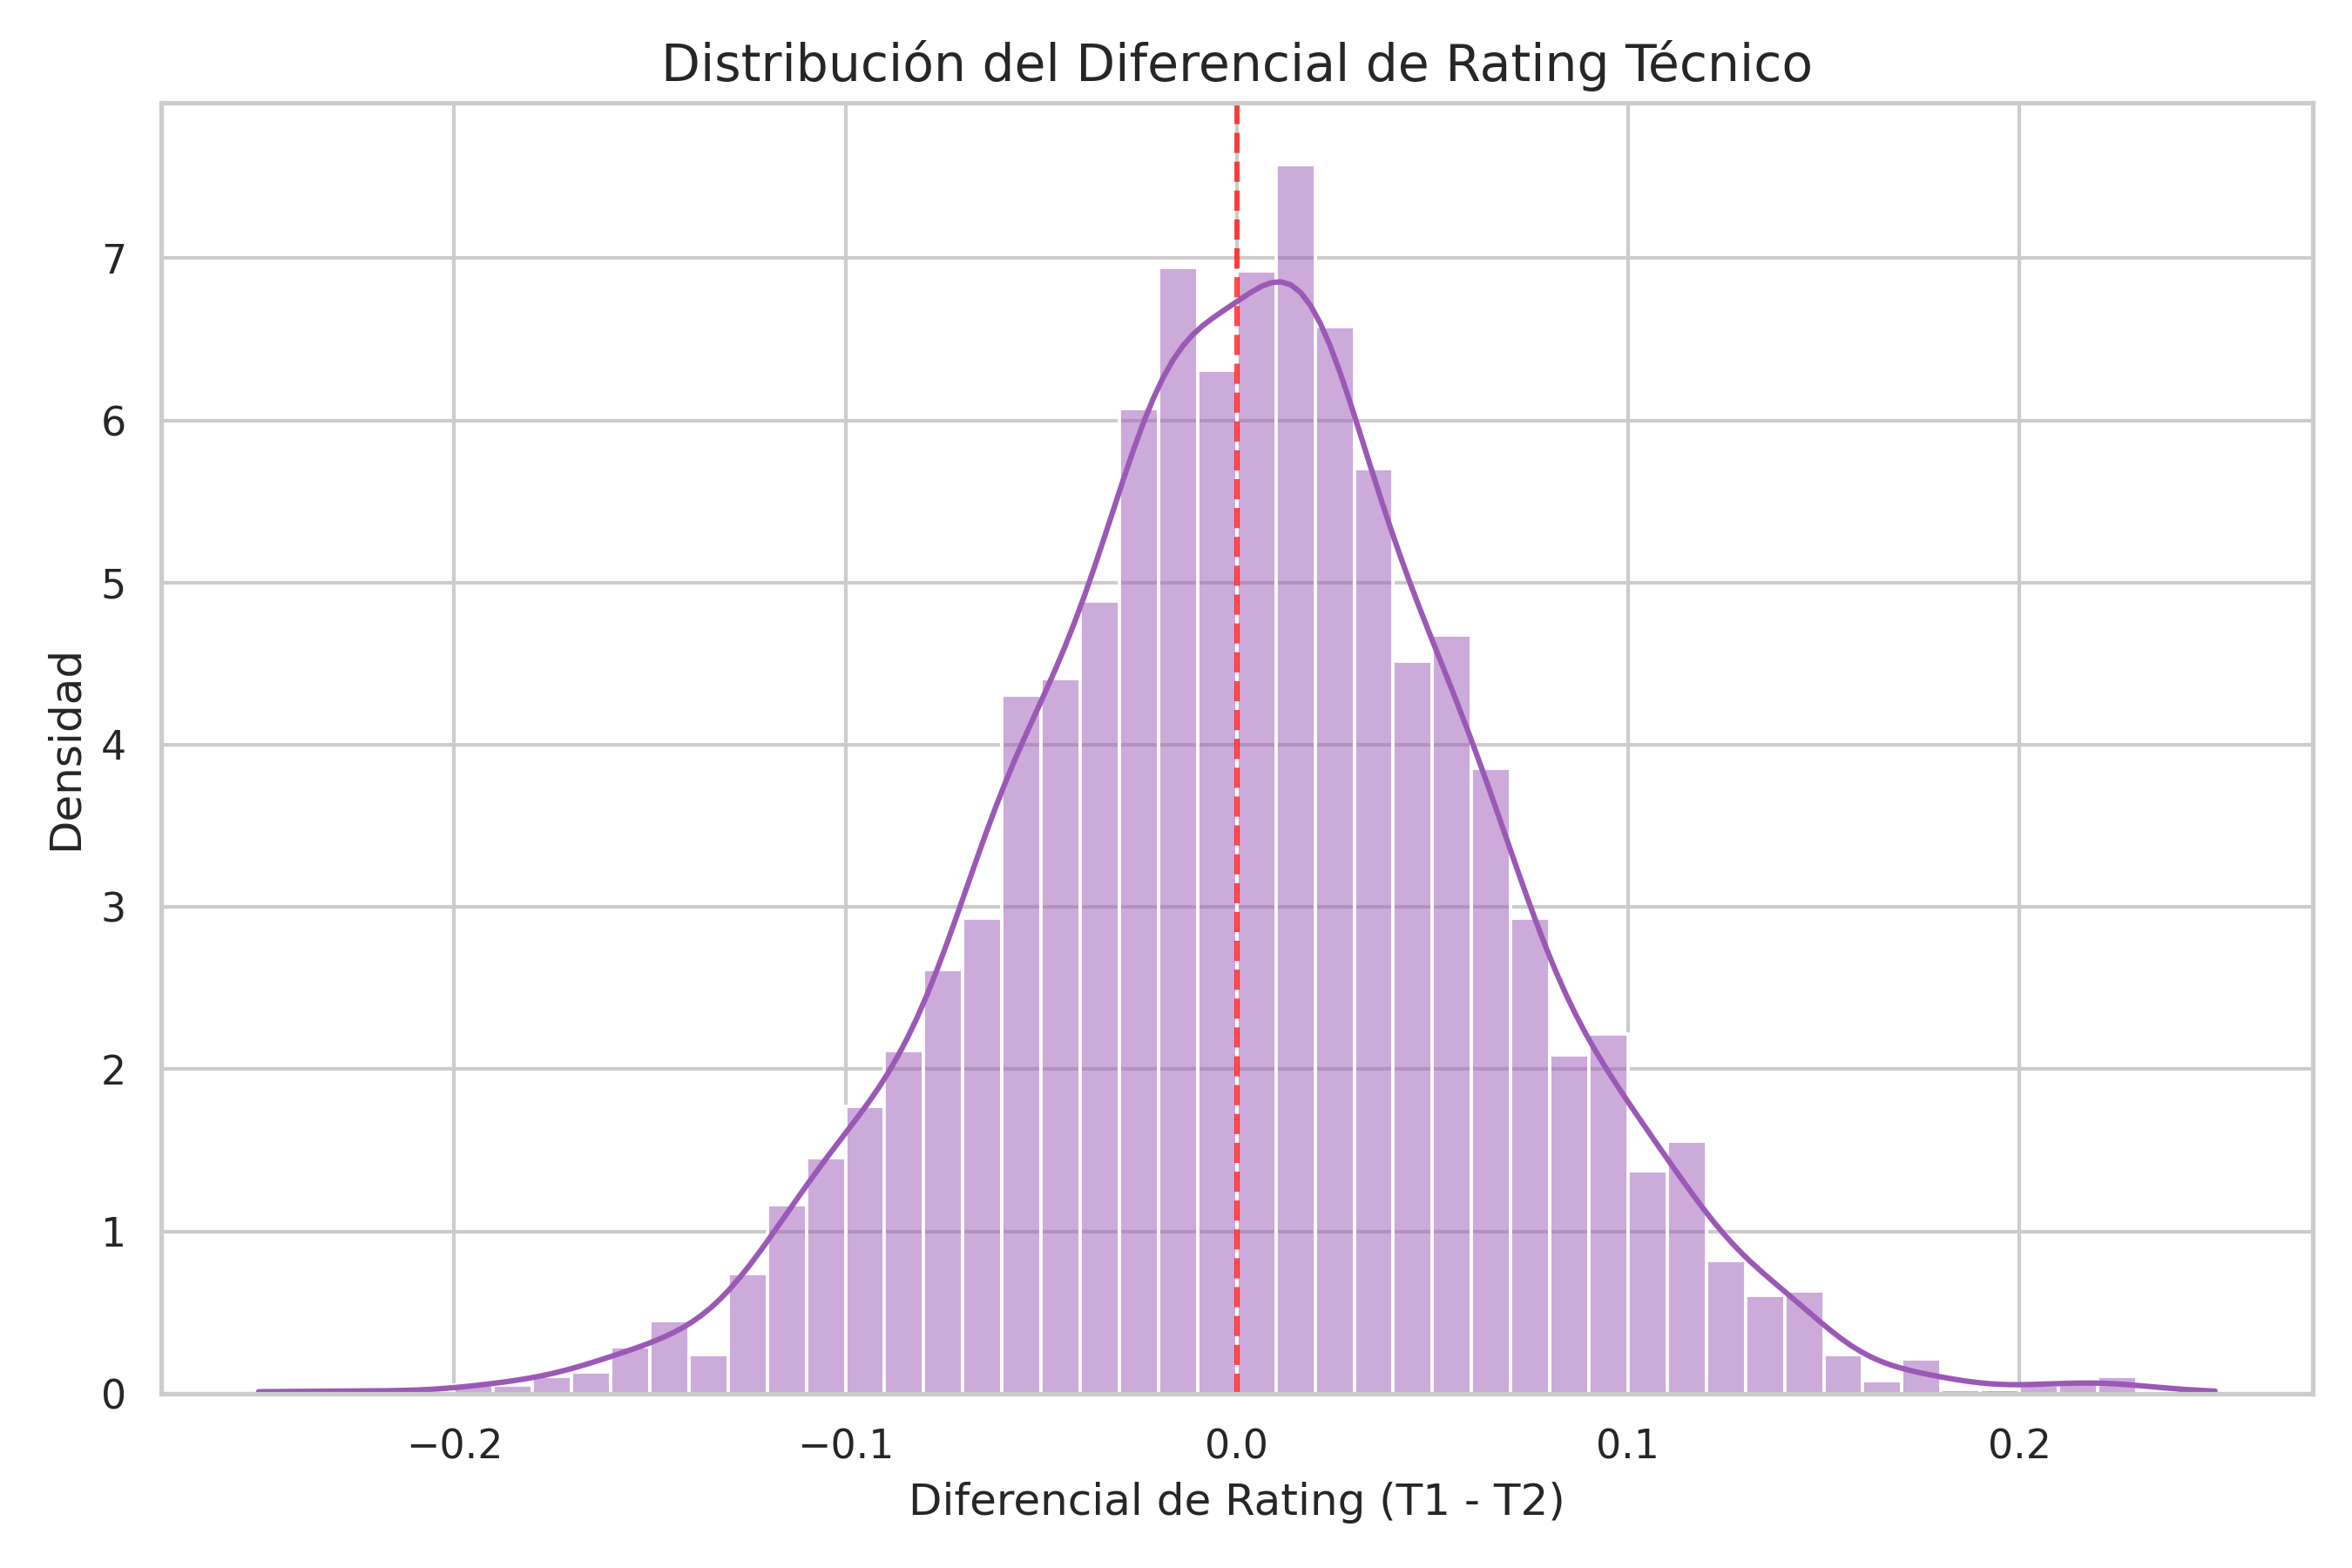
\includegraphics[width=\linewidth]{distribucion_densidad_rating.png}
    \caption{Concentración de la Habilidad. Destaca cómo la gran masa de partidos profesionales agrupa a escuadras supremamente igualadas (cerca del diferencial 0).}
    \label{fig:DistFig}
\end{figure}

Como nos enseña de forma clara la Figura \ref{fig:DistFig}, casi todos los duelos ocurren entre equipos con niveles demasiado similares (formando una pequeña campana central acentuada). Esto es justo lo que nos motivó al uso de estadística bayesiana: en cruces de vida o muerte tan parejos es vital que, antes de arrojarnos un simple pronóstico dictatorial binario, el motor nos brinde en bandeja toda el abanico palpable de asimetría o márgenes de duda que rondan dicho enfrentamiento.

\begin{figure}[H]
    \centering
    
\includegraphics[width=\linewidth]{matriz_correlacion_completa.png}
    \caption{Matriz de Correlación. Demuestra qué componente impacta más el logro de una victoria directa.}
    \label{fig:CorrFig}
\end{figure}

Al leer los colores de la interactividad vista en la Figura \ref{fig:CorrFig}, podemos enfocar nuestra fe en factores eficientes. El número que destaca por un margen monumental al indicarnos un acierto para la \textit{Victoria T1} viene siendo precisamente el peso de nuestro Diferencial de Rating (que encabeza un \textit{0.26} probabilístico), seguido discretamente por el Factor Impacto, validando por qué elegimos estos factores para que apalanquen a la máquina de inferencia.

\begin{figure}[H]
    \centering
    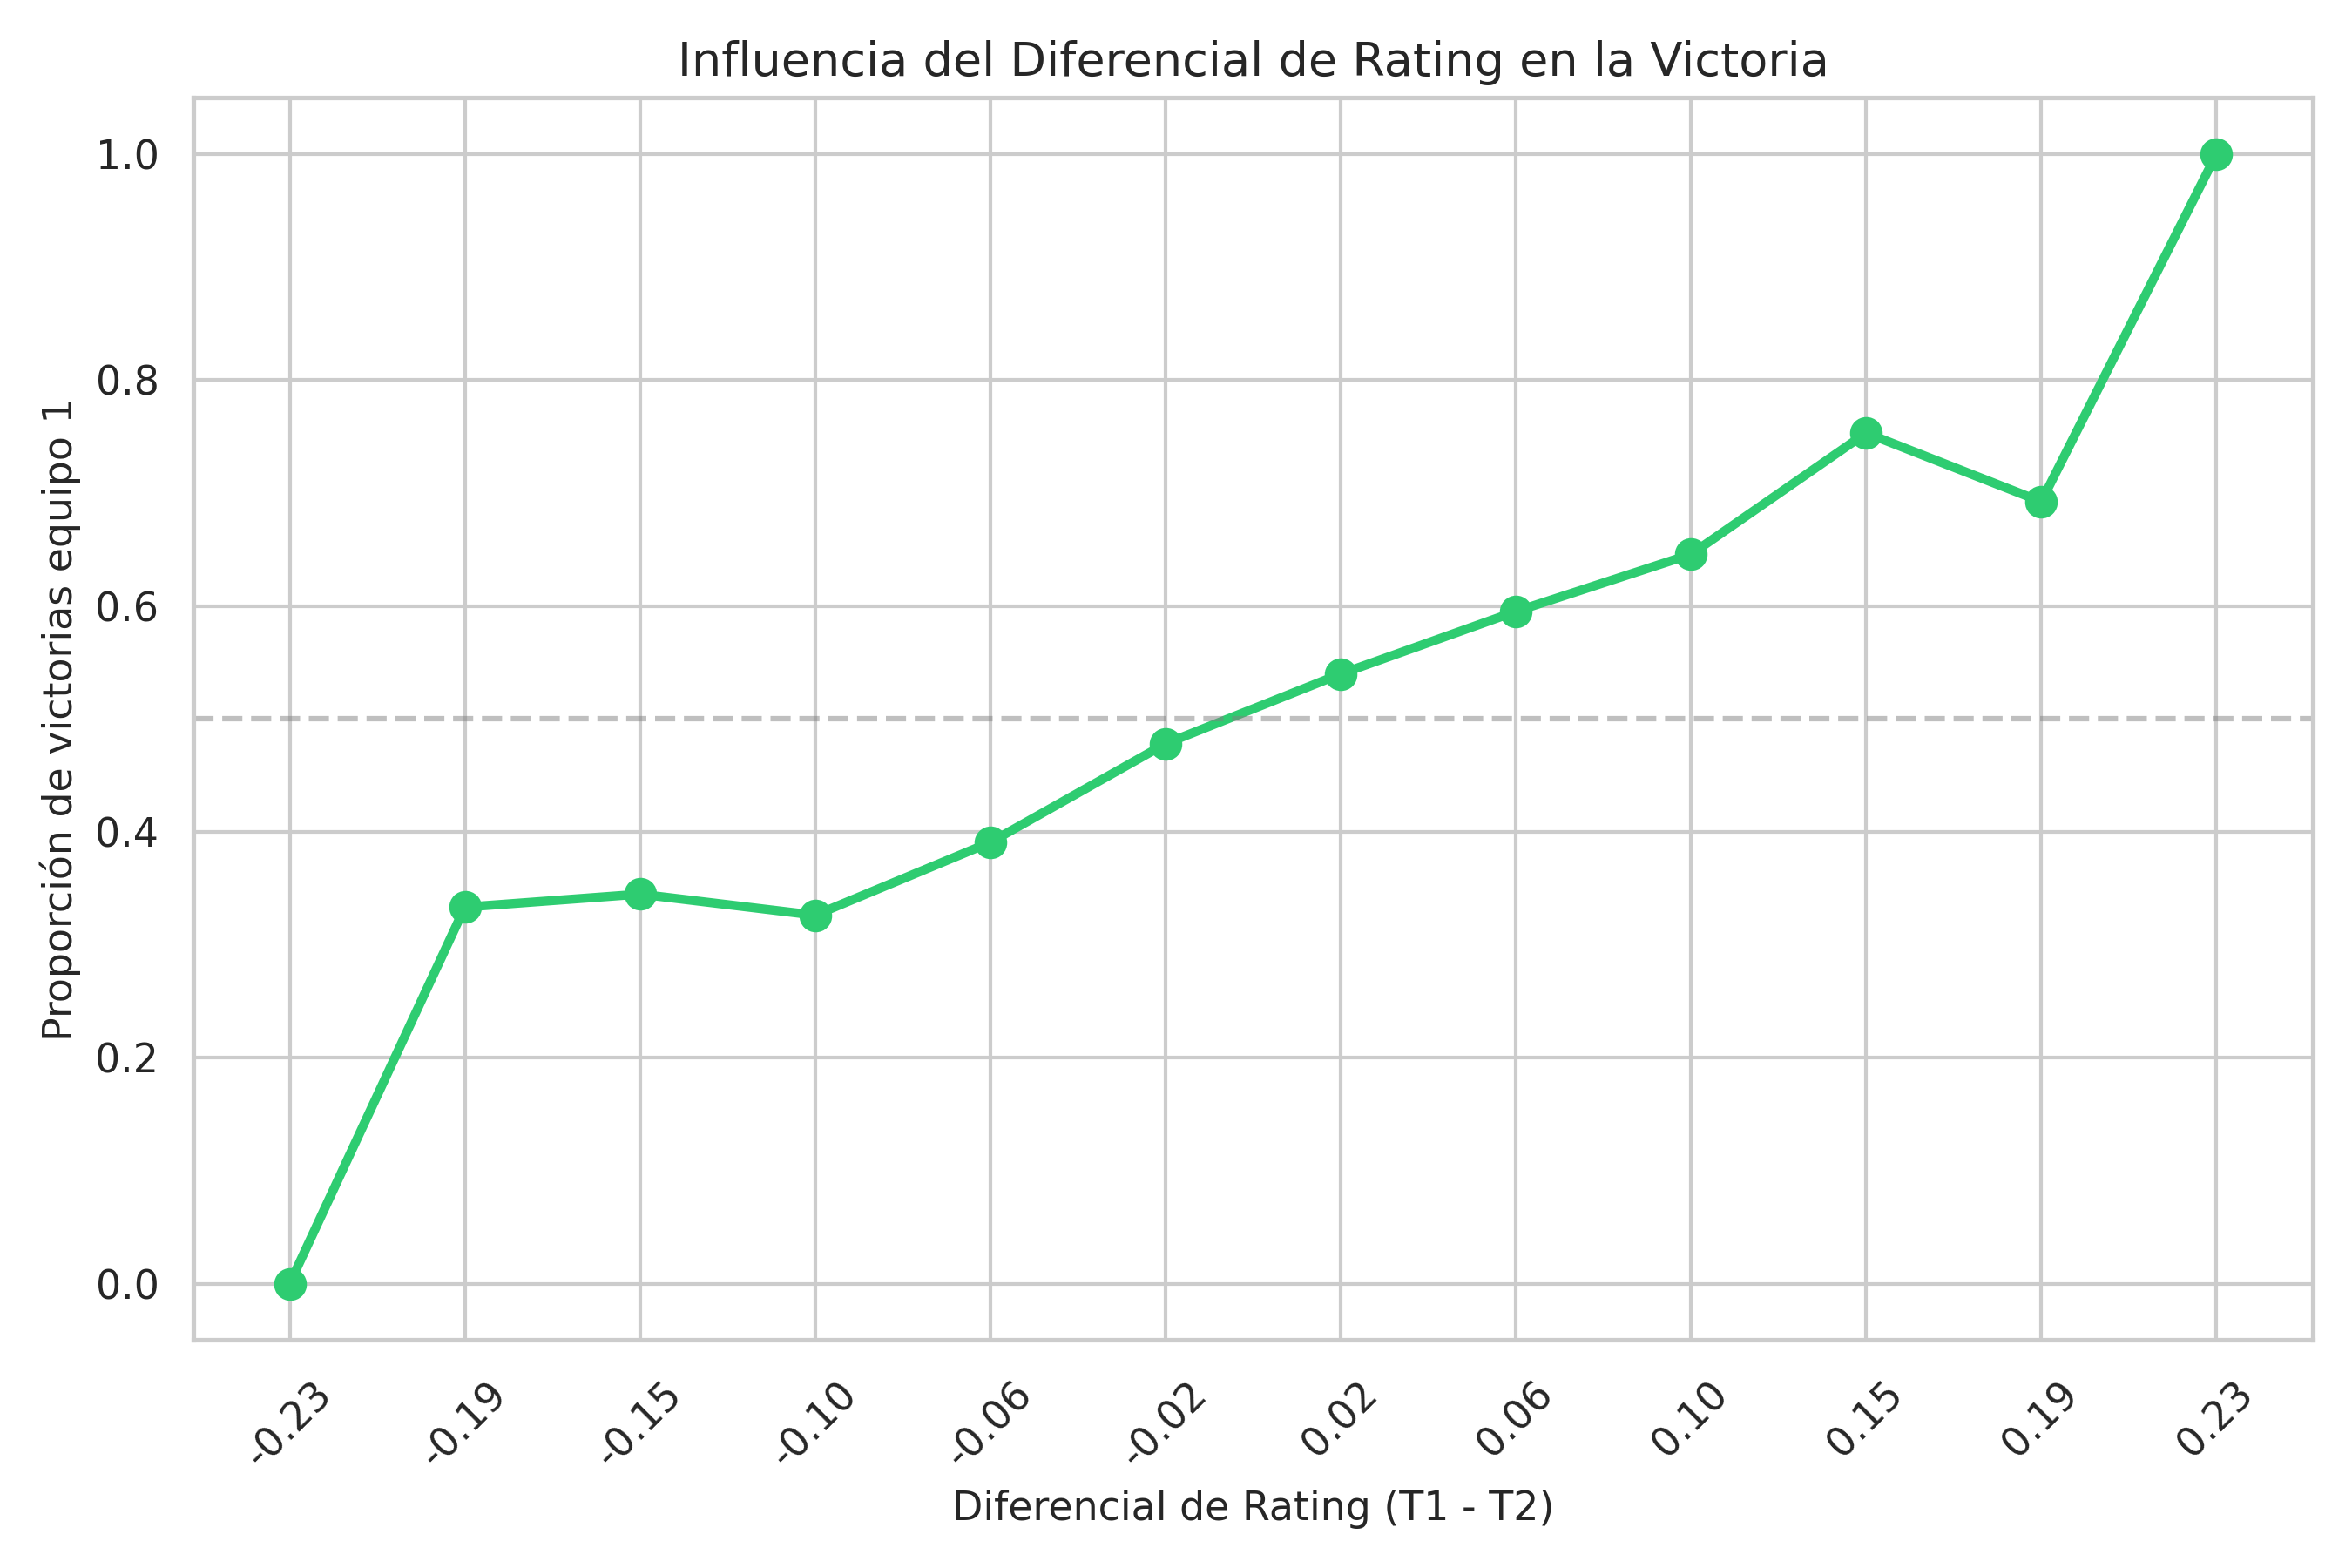
\includegraphics[width=\linewidth]{evidencia_rating_winrate.png}
    \caption{El Rating dictamina la Victoria. Queda ilustrado cómo un leve aumento constante en ventaja de talento impulsa radicalmente las posibilidades de triunfo asintóticas.}
    \label{fig:WinrateFig}
\end{figure}

En gran sintonía con nuestro proceso \textit{logit} paramétrico, es visible matemáticamente en la contundencia lineal de la Figura \ref{fig:WinrateFig} cómo la tasa natural de las victorias aumenta exponencialmente por el rating.

\begin{figure}[H]
    \centering
    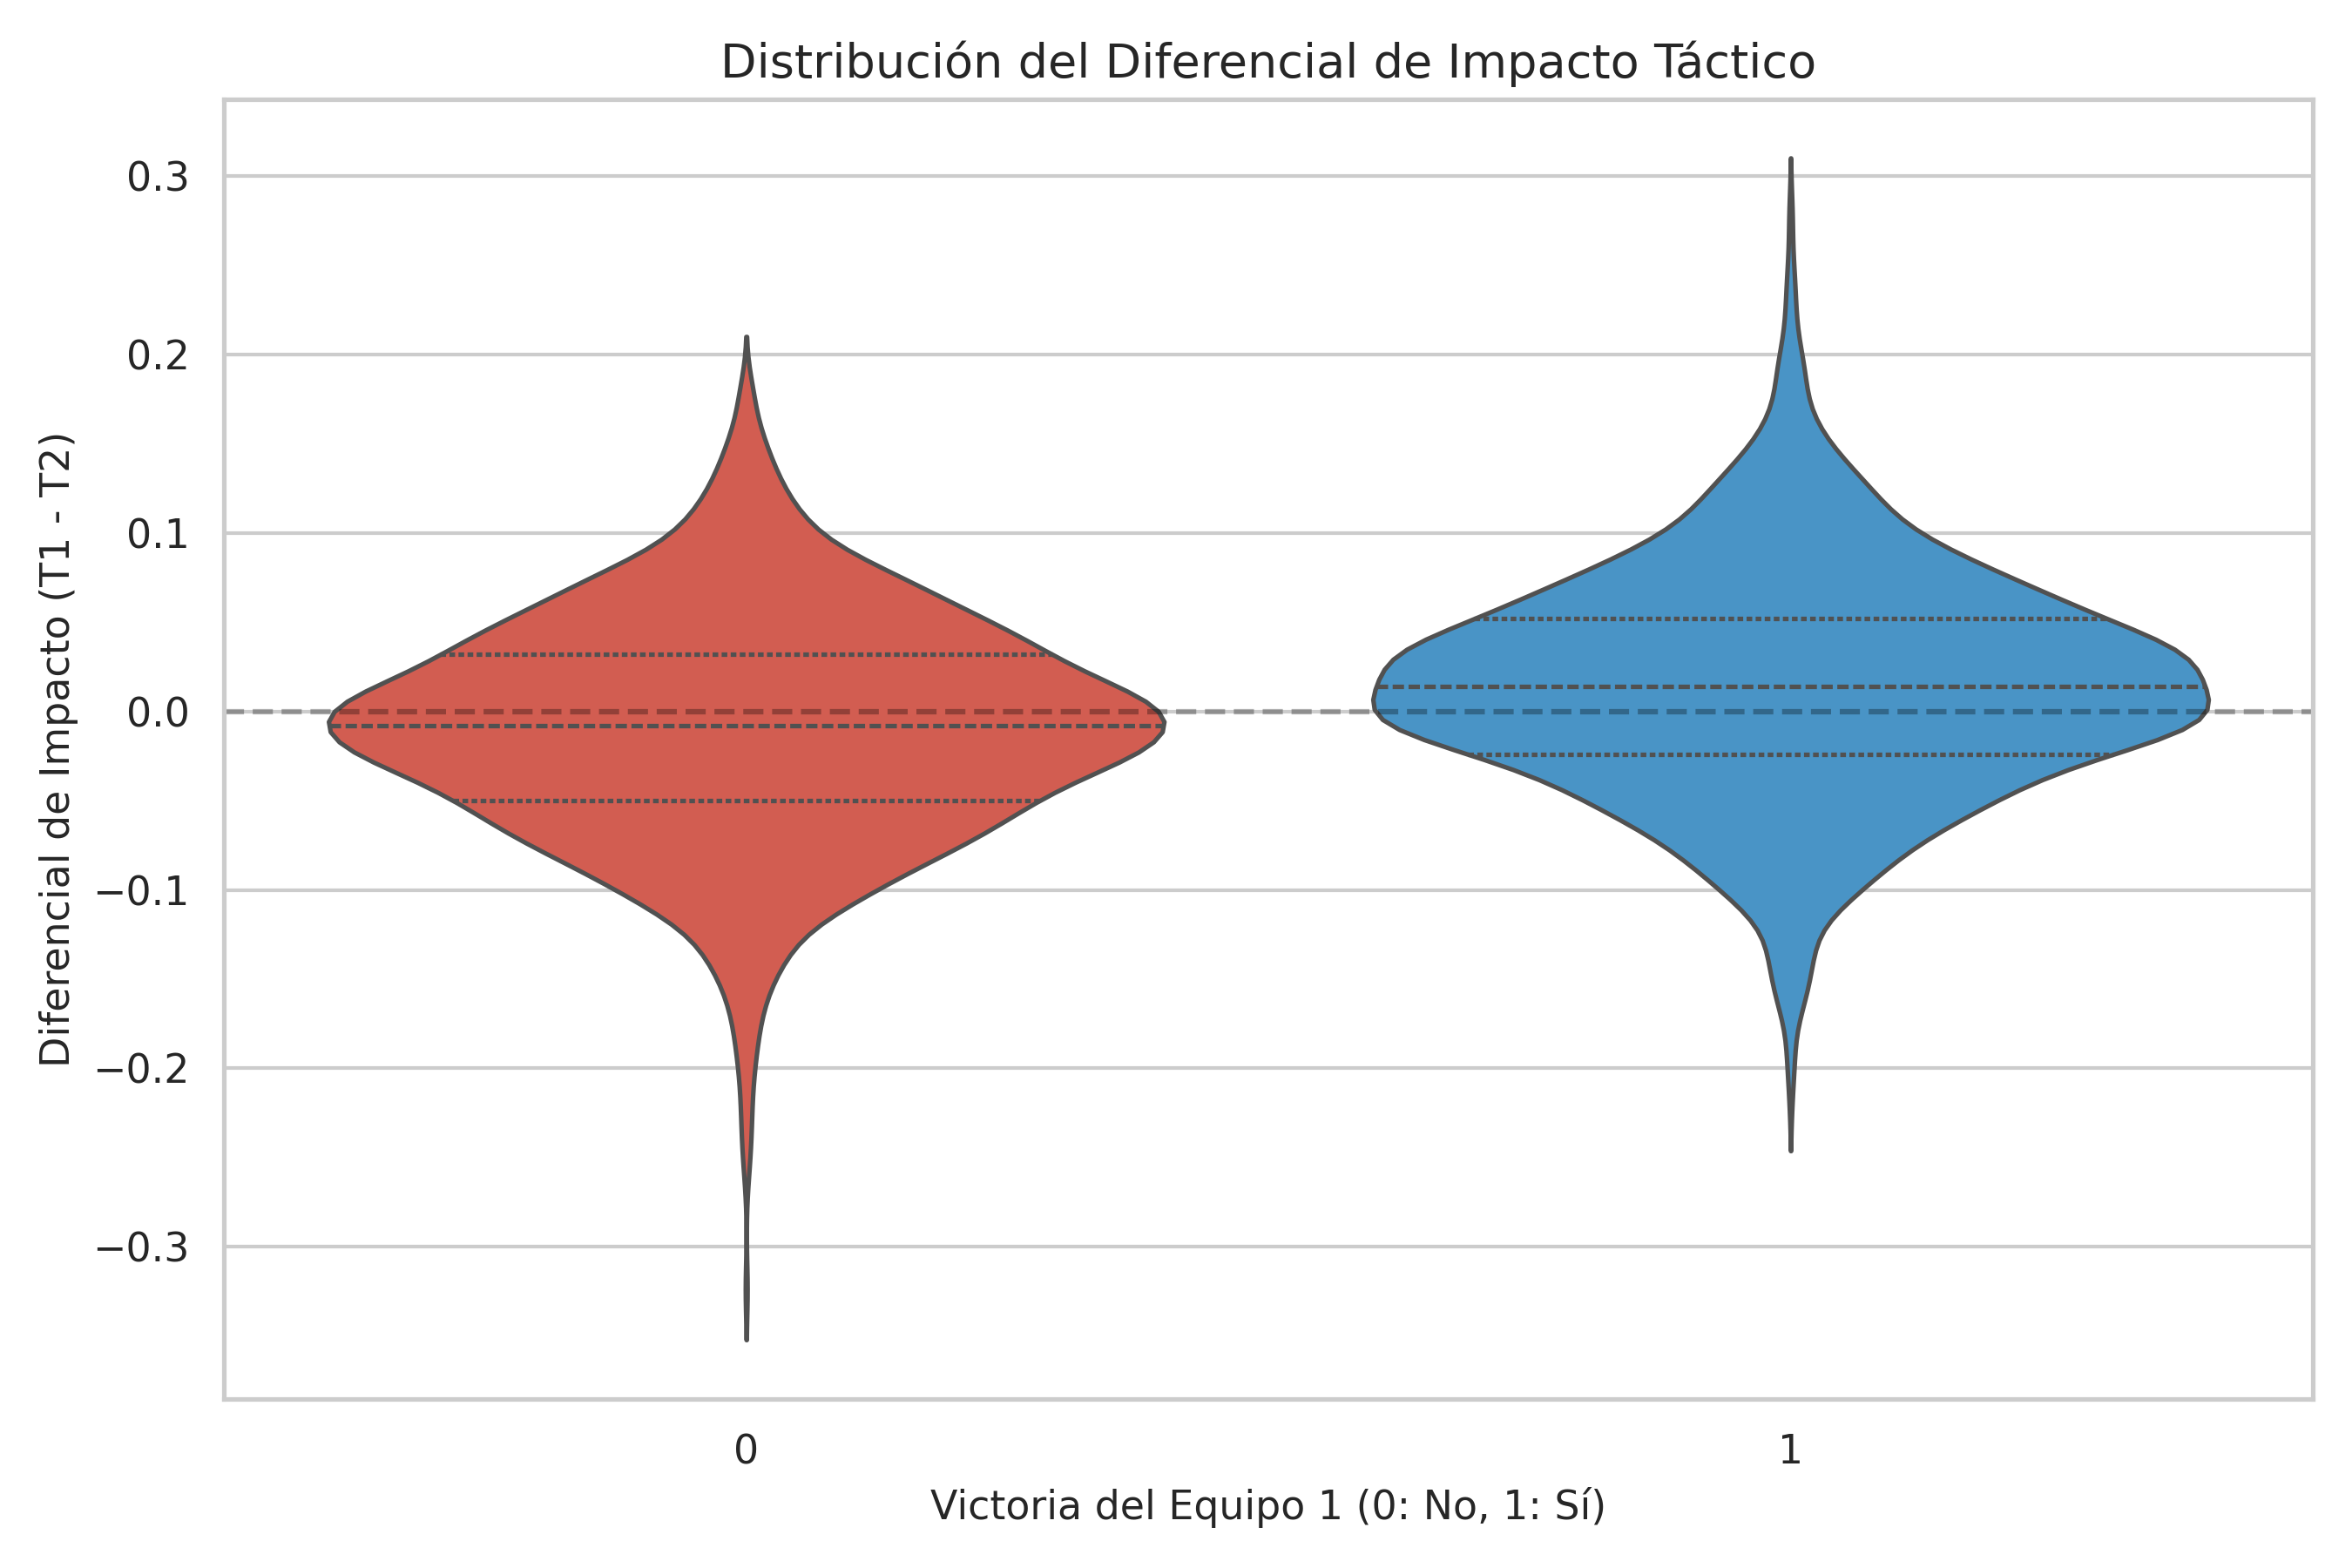
\includegraphics[width=\linewidth]{evidencia_impacto_violin.png}
    \caption{El peso Táctico. Las formaciones abultadas de la gráfica revelan gran volatilidad, es decir, el impacto decide partidas pero fluctúa salvajemente dependiendo del día de juego.}
    \label{fig:ImpactFig}
\end{figure}

Es innegable para cualquiera ver que la gran expansión en el violín (Figura \ref{fig:ImpactFig}) expone peligro y azar. El impacto nos encanta pero contiene demasiadas eventuales excepciones asimétricas, lo cual nos insta y sirve a futuro de argumento en la holgura de credibilidad que se designará.

\begin{figure}[H]
    \centering
    
\includegraphics[width=\linewidth]{balance_ct_t_mapas.png}
    \caption{El sesgo de ``Jugar Defendiendo''. En cada entorno competitivo se prueba históricamente una tasa de ganancia por bando radicalmente distinta y condicionante.}
    \label{fig:MapasFig}
\end{figure}

\subsection{Presentación de las hipótesis}
Al comprender visualmente la data obtenida y simplificarla para lo que busca nuestra investigación final, asentamos en piedra las tres expectativas formales que deseamos el modelo corrobore más adelante:

\begin{itemize}
    \item \textbf{H1 (El Peso Pesado del Rating):} Apostamos a que en encuentros donde la media en habilidad posicional mida un escalón notorio frente a quien se enfrenta, el atributo dictaminará gran parte de la tajada resolutiva de la ecuación central, empujando implacablemente las posibilidades de sobrepasar a quienes son los desfavorecidos técnicos para el juego.
    
    \item \textbf{H2 (Volatilidad Regularizada Táctica):} Consideramos que los actos de inflexión de ronda (como dobles asesinatos y entradas sorpresivas) cambiarán pronósticos de vida, pero sus intermitencias no las consideramos 100\% certeras. Esperamos que una flexibilidad amortiguada proteja el comportamiento del \textit{motor de cálculo} y evite una fe sobre-comprometida ("overfitting").
    
    \item \textbf{H3 (Terrenos Desnivelados CT/T):} Analizando cartográficamente las tendencias (Fig \ref{fig:MapasFig}), creemos crucial prever que ciertas áreas físicas alteran automáticamente la ventaja "injustamente" por defecto, conllevando directamente a que la predicción neutra pura o de neutralidad inicial requiera balances posteriores dinámicos por interceptos de variables estructurales.
\end{itemize}

\section{ESPECIFICACIONES DE LAS PRIORS (Punto 3.2.6)}

Para configurar apropiadamente el esqueleto logístico de nuestro acercamiento Bayesiano y acatar con los fines metodológicos rigurosos de nuestra materia de análisis, le inyectaremos de base al agente calculador (\textit{MCMC}) unos preceptos a los que titularemos \textbf{``Creencias Anteriores'' o Priors}. En el argot de una regresión preestablecida ($logit \sim \alpha + \beta_{rtg} + \beta_{imp}$), predefinimos y asumimos estos dictámenes paramétricos haciendo que la computadora ensaye usando de telón de control empírico un modelo histórico con el \textit{Dataset global gigante} del que estamos extrayendo valores, previo a forjar lo que será sometido a un escenario específico sin sesgos injustos.

\subsection{Definición de Nuestras Perspectivas Preestablecidas}

Explotamos a nuestro favor distintas intensidades de rigidez de creencia basadas en nuestra familiaridad para educar jerárquicamente a la máquina, las cuales estipulamos bajo el modelo estadístico tradicional Normal (campana):

\begin{itemize}
    \item \textbf{A. Prior Informativa: Habilidad Basal de Equipo ($\beta_{rating}$)}\\
    \textbf{Características Elegidas:} Normal $N(\mu = 4.79, \sigma = 1.28)$\newline
    \textbf{Justificativa Práctica:} Como lo atestiguamos de una manera tan arrolladora en el gráfico de su línea de tracción (Figura \ref{fig:WinrateFig}), dictaminamos total fe y resguardo posicional aquí. Reaccionar en la paramétrica aplicándole tan corto renglón de flexibilidad o encogimiento ($\sigma = 1.28$) se interpreta humanamente en que, de base, le cerramos las puertas mentales a nuestro agente matemático permitiéndole enfrascarse y sostener fe inercial asfixiando desviaciones: el \textit{rating alto gana partidas irremediablemente}.
    
    \item \textbf{B. Prior Débilmente Informativa: Factor Operativo de Impacto ($\beta_{impact}$)}\\
    \textbf{Características Elegidas:} Normal $N(\mu = 1.99, \sigma = 5.00)$\newline
    \textbf{Justificativa Práctica:} Estamos conscientes de que este factor empuja y beneficia considerablemente el vector de éxito del conjunto que esté arriba ($1.99$), pero sus violines mostraron oscilaciones difusas para rondas clave. Decidimos asignarle de base aquí un abanico enorme o esparcido de fluctuaciones ($\sigma = 5.00$), una flexibilización que actúa a modo de \textit{amortiguador transigente psicológico} para el software, con ello, confía a medias pero tiene soberanía gigante y maleabilidad para aprender empíricamente sobre el terreno o dudar dictatorialmente.
    
    \item \textbf{C. Prior No Informativa: Perfil Base o Intercepto Equilibrado ($\alpha$)}\\
    \textbf{Características Elegidas:} Normal $N(\mu = 0.01, \sigma = 100.0)$\newline
    \textbf{Justificativa Práctica:} Entramos en una postura de agnosticismo pleno de no dar un duro por nadie. Si abstrajéramos de la ecuación al mapa asimétrico y dictámenes de talento de pre-juego, asentaríamos una planitud o desviación colosal ($\sigma = 100$). En un dibujo general, anula todo chances de conferir por obviedad imperativa naturalista un ventajismo injustificado sin un previo rastreo cruzado, asegurando por sí misma imparcialidad probabilística.
\end{itemize}

\subsection{Contrastación Funcional de Espectros Paramétricos}

Al ilustrar un super-encaje o vista gráfica directa de los resultados de credibilidad con los que jugaremos tras la orquestación (Figura \ref{fig:PriorsComp}), desvelamos visualmente toda la configuración de arranque lista para la experimentación por cadenas de Markov de siguientes partes de entrenamiento.

\begin{figure}[H]
    \centering
    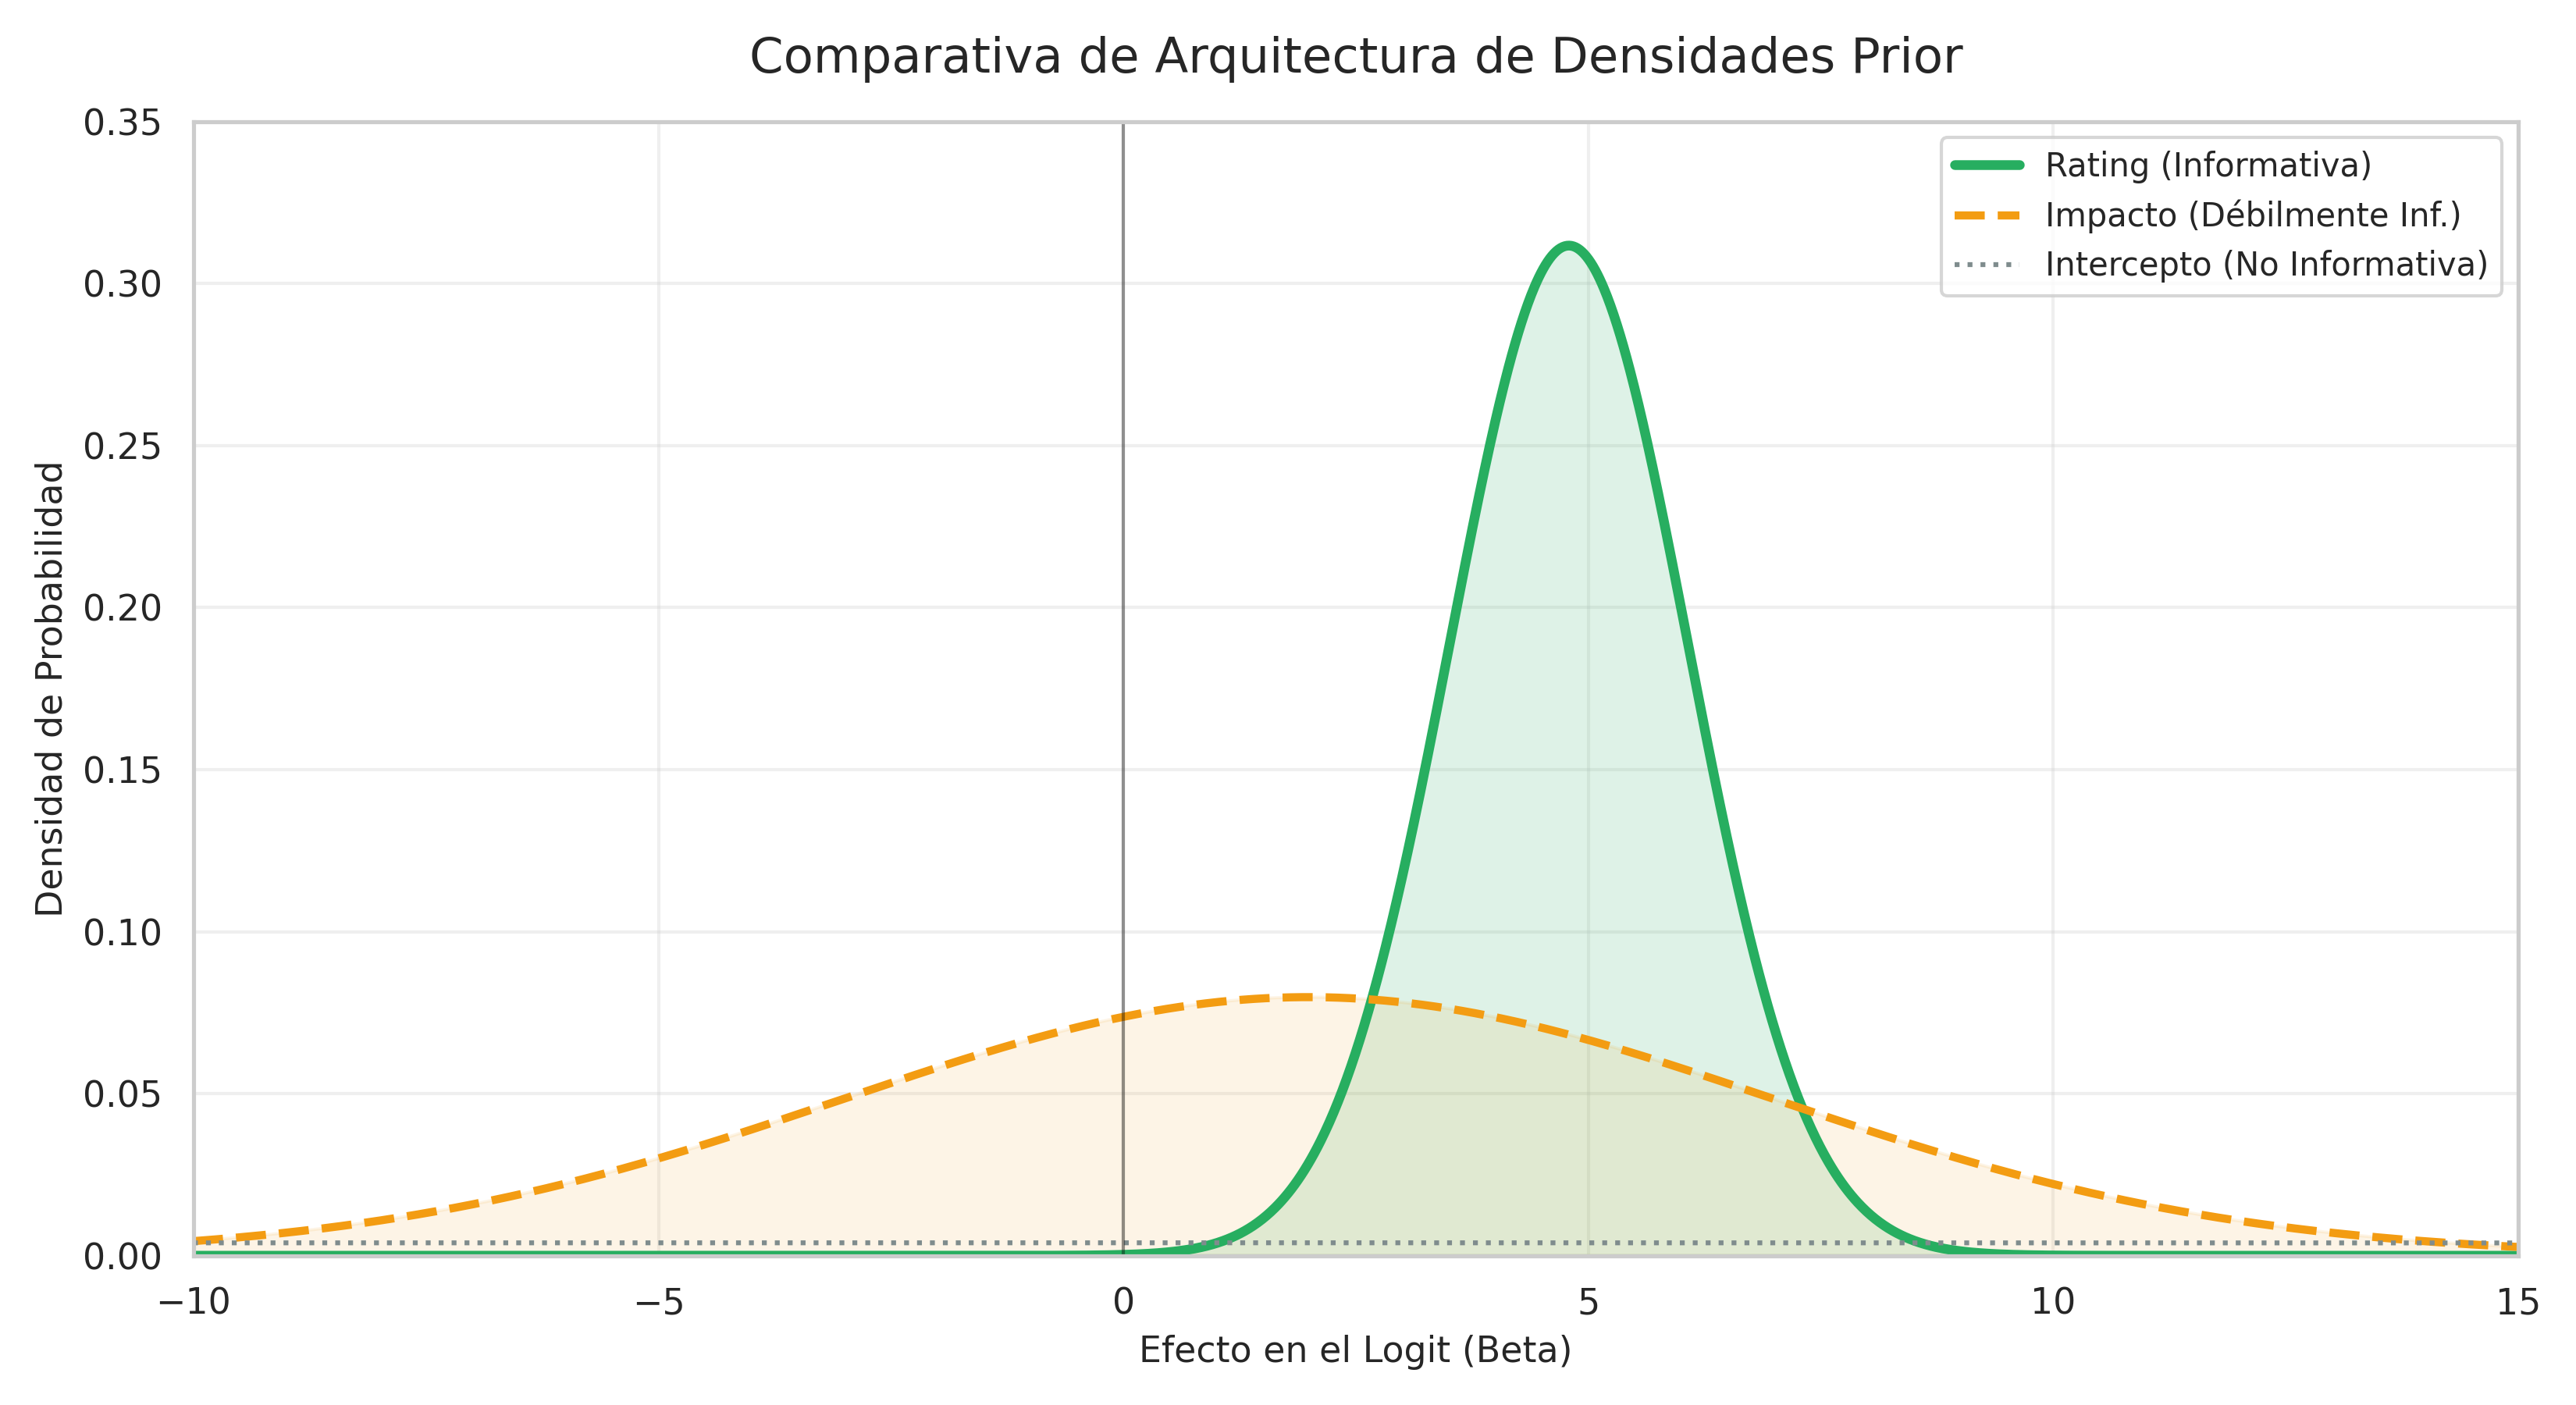
\includegraphics[width=\linewidth]{comparativa_priors.png}
    \caption{Contrastación Emparedada entre Priors. En verde fuerte, los datos del Rating posan erguidos como picos dictando "información de altísimo compromiso". Paralelamente, la capa táctica amarrilla divaga achatada por una prudencia permisiva asignada; por contraste, la sutileza final representa el terreno agnóstico estadístico al que no le importa el status previo a analizar.}
    \label{fig:PriorsComp}
\end{figure}

Entendemos de forma palpable que sería bastante desacertado como científicos forzarle a toda mecánica virtual un rigor y severidad tiránica desmedida sobrepasando su historial natural. Conducir a un premio o encierre sobre métricas firmes, pero paralelamente entregarle amabilidad adaptativa e impunidad analítica para las métricas volátiles, evitará sustos clásicos que arruinan la estabilidad predictiva final a un \textit{Machine Learning} regularizado.

\newpage
\nocite{*}
\bibliographystyle{apalike}
\bibliography{bibliografia}
\end{document}
